\chapter{Architecture and Design}\label{design}

\section{Architecture}

The architecture of the project is structured into the import phase (ETL process), the changed tiles detection phase  and the export phase (render vector tiles). This section describes the components and their purpose.

\begin{figure}[H]
  \centering
  \includegraphics[width=1.0\textwidth]{images/etl_components}
  \caption{Workflow structured into components}
\end{figure}

Each component is a Docker image\cite{docker} with a single purpose. The Docker containers (components) are then linked against the database container and provided with additional input data to perform their functions. Isolating the components into Docker images makes it possible to ensure that the complicated installations and dependencies of some components never cause an issue. By additionally using Docker Compose it is possible to define the entire ETL process with different containers and make deployment and scaling containers easy.

\subsection{Import Components}

The import components take care of importing \osm{} data, external data sources and SQL utilities such as views, triggers, indices and functions to help with the rendering and changed tiles detection process.

\subsubsection{Import External}

The \textbf{import-external} component is responsible for importing all data that is not mapped directly from \osm{} into the PostGIS database. \autoref{import_external_diagram} shows the external data sources and programs used to import the data into the PostGIS database. The GDAL tool ogr2ogr is used to import the various data sources into the PostGIS database.

\begin{figure}[H]
  \centering
  \includegraphics[width=1.0\textwidth]{images/architecture/import_external_diagram}
  \caption{Import of external data sources}
  \label{import_external_diagram} 
\end{figure}

\subsubsection{Import OSM}

The \textbf{import-osm} component takes the first PBF file in the import folder and imports it into PostGIS. After that it updates the scaleranks using Natural Earth data from \texttt{import-external} to update the scaleranks and create generalized tables based off the imported data. The data is imported using imposm3 diff mode and can take up to 14 hours for the entire planet file.

\begin{figure}[H]
  \centering
  \includegraphics[width=1.0\textwidth]{images/architecture/import_osm_diagram}
  \caption{Import OSM diagram}
\end{figure}

\subsubsection{Import SQL}

The \textbf{import-sql} component is responsible for provisioning the SQL used in the different layers. It also generates SQL code for different classifications and code to detect changed tiles as well as table management commands for different layers.

\begin{figure}[H]
  \centering
  \includegraphics[width=1.0\textwidth]{images/architecture/import_sql_diagram}
  \caption{Import SQL diagram}
\end{figure}

\subsection{Changed Tile Detection Components}

The changed tile detection components handle creating an \osm{} Diff file based on a certain \osm{} planet file, importing a \osm{} Diff file and updating outdated \osm{} planet file with the latest changes. The following sections show what happens in every component.

\subsubsection{Update OSM Diff}

The \textbf{update-osm-diff} component takes the planet file as input and creates an \osm{} Diff file containing all the changes happened since the planet file was downloaded. The \texttt{osmupdate} tool is used to execute this task.

\begin{figure}[H]
  \centering
  \includegraphics[width=1.0\textwidth]{images/architecture/update_osm_diff_diagram}
  \caption{Update OSM Diff diagram}
\end{figure}

\subsubsection{Import OSM Diff}

The \textbf{import-osm-diff} component takes the \osm{} diff file created with the \textbf{update-osm-diff} component as input and imports all changes into the database.

\begin{figure}[H]
  \centering
  \includegraphics[width=1.0\textwidth]{images/architecture/import_osm_diff_diagram}
  \caption{Import OSM Diff diagram}
\end{figure}

\subsubsection{Merge OSM Diff}

The \textbf{merge-osm-diff} component takes the old planet file and the latest diff file as input and merges all changes into the old planet file. Additionally the timestamp of the planet file is updated in order to have a correct diff file when the \textbf{update-osm-diff} process runs the next time. The \texttt{osmconvert} tool is used to merge the latest diff file into the old planet file.

\begin{figure}[H]
  \centering
  \includegraphics[width=1.0\textwidth]{images/architecture/merge_osm_diff_diagram}
  \caption{Merge OSM Diff diagram}
\end{figure}

\subsubsection{Changed Tiles}

The \textbf{changed-tiles} component is responsible for executing the changed tiles SQL logic and store the list of changed tiles in a text file using pgclimb. The actual logic for detecting the changed tiles is contained in the \textbf{import-sql} component.

\begin{figure}[H]
  \centering
  \includegraphics[width=1.0\textwidth]{images/architecture/changed_tiles_diagram}
  \caption{Changed Tiles diagram}
\end{figure}

\subsection{Distributed Tile Rendering Components}

In order to meet the performance requirements a distributed rendering architecture 
is needed to scale the process on to multiple hosts and process. The central component of the rendering pipeline is the message queue which contains the rendering jobs and results all other components interact with the message queue to take or confirm a job.

\subsubsection{Generate Jobs}

The \texttt{generate-jobs} component is responsible for creating JSON jobs consumed by the \texttt{export} component. It supports two types of jobs:

\begin{itemize}
  \item \textbf{Pyramid}: Job of rendering a tile pyramid (e.g. from z8 all down to z14). Used for initial rendering of the world.
  \item \textbf{List}: Batch jobs of list of tiles to be rendered grouped by data locality. Used for rendering changed tiles.
\end{itemize}

Generate-jobs will output the jobs as individual JSON objects to stdout. A tool like \texttt{pipecat} can be used to schedule them on the job server.

\begin{figure}[H]
  \centering
  \includegraphics[width=1.0\textwidth]{images/architecture/generate_jobs_diagram}
  \caption{Generate Jobs diagram}
\end{figure}
\clearpage

\subsubsection{Export}

The \textbf{export} component is responsible for rendering vector tiles using osm2vectortiles.tm2source and the \textbf{postgis} component. Exports can be run together with a message queue like RabbitMQ or standalone for smaller extracts where it is not necessary to divide the work into several parts.

\begin{figure}[H]
  \centering
  \includegraphics[width=1.0\textwidth]{images/architecture/export_worker_diagram}
  \caption{Export Worker diagram}
\end{figure}

\subsubsection{Merge Jobs}

The \textbf{merge-jobs} component is responsible for taking result messages from the queue, download the attached MBTiles file and merge it into the latest planet MBTiles file.

\begin{figure}[H]
  \centering
  \includegraphics[width=1.0\textwidth]{images/architecture/merge_jobs_flow_diagram}
  \caption{Merge Jobs diagram}
\end{figure}

%------------------------------------------------------
\section{Database and Layer Schema}\label{database-schema}

In this section the different layers and the database schema related to it are explained and justified. Each layer contains a diagram showing the relations and model between tables, zoom level views (\autoref{zoom_level_views}) and the vector tile layers (\autoref{layer_diagram_notation}).
The database schema is denormalized and has no relations to fulfill the performance constraints of rendering.
It is heavily optimized for fast reads since the only use case of the database schema is generating vector tiles from the PostGIS database.


\begin{figure}[H]
  \centering
  \includegraphics[width=0.8\textwidth]{images/diagram_notation}
  \caption{Database and layer schema diagram notation}
  \label{layer_diagram_notation}
\end{figure}

%------------------------------------------------------
\subsection{Barriers}

\noindent\begin{minipage}[t]{0.48\linewidth}
    \vspace{0pt}
    The layer \textbf{barrier\_line} contains barriers that block a way or path. Common features are structural walls, fences or access controls like bicycle barriers and gates. Man made objects like piers or natural barriers like a cliff are contained as well in the \textbf{barrier\_line} layer. Barriers are quite a detailed information and are therefore only relevant at the highest zoom level 14.
\end{minipage}
\hfill
\begin{minipage}[t]{0.48\linewidth}
    \begin{figure}[H]
      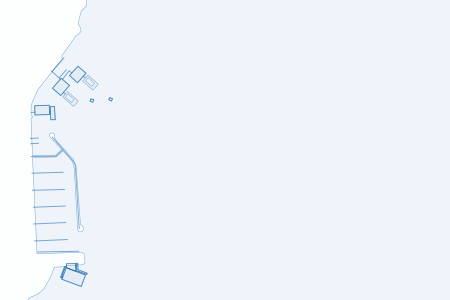
\includegraphics[width=1\textwidth]{images/schema/piers_example}
      \caption{Barrier line layer with piers}
    \end{figure}
\end{minipage}

\begin{figure}[H]
  \centering
  \includegraphics[width=0.8\textwidth]{images/schema/barrier_line}
  \caption{Barrier layer}
\end{figure}


%------------------------------------------------------
\subsection{Water}


\noindent\begin{minipage}[t]{0.48\linewidth}
    \vspace{0pt}
    The \textbf{water} layer contains bodies of water like the ocean, lakes or large rivers.
    Since water is essential to the quality of the map different data sources as shown in \autoref{water_data_sources_table} are used on different zoom levels. 
    The \textbf{water\_label} layer shows the labels of lake bodies (not marine waters). Due to the costly calculation of centroid of very large polygons the \textbf{water\_point} table is precalculated ahead of rendering time.
    \\\\
    Coastlines in \osm{} are sensitive for change and
    the OpenStreetMapData\cite{14_openstreetmapdata.com_2015}
    project takes care of repairing broken coastlines and checking it thoroughly. The OpenStreetMapData project also takes care of splitting the ocean into several smaller tiled polygons which results in better database performance.
    The \textbf{water} layer uses simplified ocean polygons from \textbf{osm\_ocean\_polygon\_gen0} on zoom level 4 and the original polygons from \textbf{osm\_ocean\_polygon} are used from zoom level 5 up to zoom level 14.
    \\\\
    For choosing the right water bodies at low zoom levels the NaturalEarth data set \cite{16_naturalearthdata.com_2015} provides manually curated data of physical features such as water in the Shapefile format. For lakes and oceans water polygons of different resolutions (1:110M, 1:50M and 1:10M) were chosen on zoom level 0 to 4.
\end{minipage}
\hfill
\begin{minipage}[t]{0.48\linewidth}
    \vspace{-10pt}
    \begin{figure}[H]
      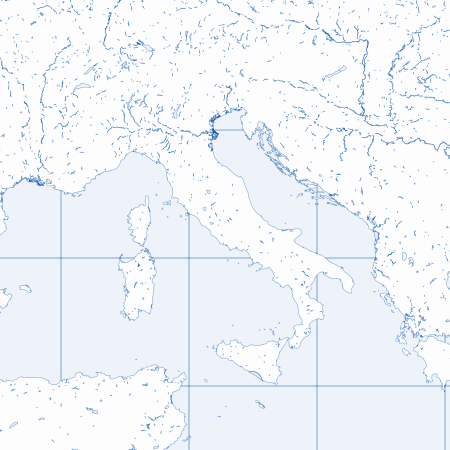
\includegraphics[width=1\textwidth]{images/schema/water_example}
      \caption{Ocean and water polygons in southern Europe}
    \end{figure}
    
    \begin{table}[H]
    \centering
        \scalebox{0.9}{
            \begin{tabular}{lll}
            \hline
            Table Name                    & Source            \\
            \hline
            ne\_110m\_ocean               & NaturalEarth      \\
            ne\_110m\_lakes               & NaturalEarth      \\
            ne\_50m\_ocean                & NaturalEarth      \\
            ne\_50m\_lakes                & NaturalEarth      \\
            ne\_10m\_ocean                & NaturalEarth      \\
            ne\_10m\_lakes                & NaturalEarth      \\
            osm\_ocean\_polygon\_gen0     & OpenStreetMapData \\
            osm\_ocean\_polygon           & OpenStreetMapData \\
            \end{tabular}
        }
        \caption{Tables from external data sources for water layer}
        \label{water_data_sources_table}
    \end{table}
\end{minipage}

\begin{figure}[H]
  \centering
  \includegraphics[width=0.8\textwidth]{images/schema/water}
  \caption{Water layer schema}
\end{figure}
    

%------------------------------------------------------
\subsection{Roads}

\noindent\begin{minipage}[t]{0.48\linewidth}
    \vspace{0pt}
    Roads are one of the most essential features in maps. Roads are present across all zoom levels filtered by type. At the lowest zoom levels only motorways are shown while at higher zoom levels residential and service roads are rendered as well. Due to the complex hierarchy of roads in \osm{} each zoom level contains custom filters to control which kind of roads get displayed on which zoom level. The \textbf{road} and \textbf{road\_label} layer, query the data from the \textbf{road\_geometry} table where both linestrings and polygons (for bigger avenues and squares) are present.
    The \textbf{road\_label} layer consists of linestrings with a road name assigned and the vector tile client then takes care of drawing the road label text across the road linestring. To avoid having too many labels on roads (especially relevant for motorway signs) the roads are grouped by their vicinity and ranked by their length to reduce label density.
\end{minipage}
\hfill
\begin{minipage}[t]{0.48\linewidth}
    \vspace{-10pt}
    \begin{figure}[H]
      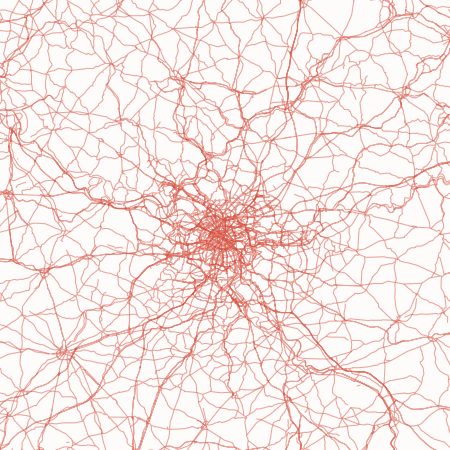
\includegraphics[width=1\textwidth]{images/schema/road_example}
      \caption{Road layer around Paris}
    \end{figure}
\end{minipage}

\begin{figure}[H]
  \centering
  \includegraphics[width=0.8\textwidth]{images/schema/road}
  \caption{Road layer schema}
\end{figure}



%------------------------------------------------------
\subsection{Buildings and Housenumbers}

\noindent\begin{minipage}[t]{0.48\linewidth}
    \vspace{0pt}
    Buildings are polygons such as houses or skyscrapers. They only appear on the highest zoom level 14 with the exception of large buildings already appearing at zoom level 13. Buildings are one of the most frequent features at high zoom levels.
    
    The \textbf{housenum\_label}  layer contains buildings or single points tagged with a housenumber. Housenumbers only appear on zoom level 14.

\end{minipage}
\hfill
\begin{minipage}[t]{0.48\linewidth}
    \vspace{-20pt}
    \begin{figure}[H]
      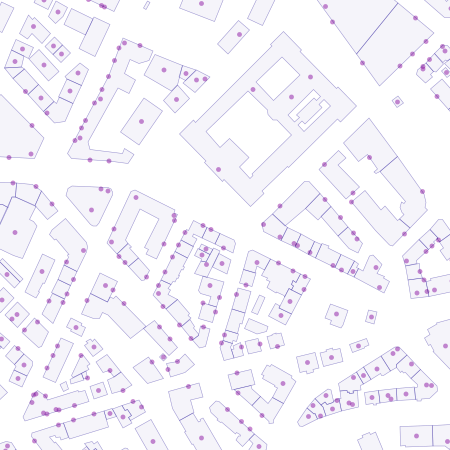
\includegraphics[width=1\textwidth]{images/schema/building_example}
      \caption{Buildings and house numbers}
    \end{figure}
\end{minipage}

\begin{figure}[H]
  \centering
  \includegraphics[width=0.8\textwidth]{images/schema/building}
  \caption{Building layer schema}
\end{figure}

%------------------------------------------------------
\subsection{Administrative Boundaries}

\noindent\begin{minipage}[t]{0.48\linewidth}
    \vspace{0pt}
    The \textbf{admin} layer contains the linestrings of administrative boundaries such as countries, states or provinces.
    Boundaries are treated as linestrings because borders often break in \osm{} and can no longer be reconstructed as polygons. Therefore it is safer to work with linestrings even though this provides less cartographic styling options.
    \\\\
    Since a different level of detail is required at different zoom levels the cultural data set from  Natural Earth \cite{16_naturalearthdata.com_2015} has been used at low zoom levels for boundaries of countries, provinces and disputed areas while at higher zoom levels the more accurate \osm{} data is used.
\end{minipage}
\hfill
\begin{minipage}[t]{0.48\linewidth}
    \vspace{-20pt}
    \begin{figure}[H]
      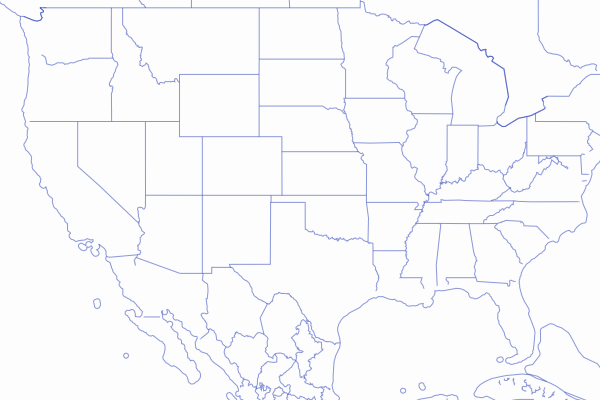
\includegraphics[width=1\textwidth]{images/schema/admin_example}
      \caption{Admin level 4 (states) in the US}
    \end{figure}
\end{minipage}

\vspace{20}

\begin{figure}[H]
  \centering
  \includegraphics[width=1\textwidth]{images/schema/admin}
  \caption{Admin layer schema}
\end{figure}

%------------------------------------------------------
\subsection{Landuse and Landuse Overlay}

\noindent\begin{minipage}[t]{0.48\linewidth}
    \vspace{0pt}
    The layer \textbf{landuse} contains polygons of specially zoned land. The most frequent 
    features inside \textbf{landuse} are wood areas as well as national parks, swamps, commercial, industrial and military zones.
    Very large polygons are split into several pieces into the \textbf{landuse\_split\_polygon} table and large polygons are generalized
    for lower zoom levels. The polygons in the \textbf{landuse} layer are filtered by area depending on the zoom level so that at low zoom levels only the biggest polygons are shown.
\end{minipage}
\hfill
\begin{minipage}[t]{0.48\linewidth}
    \vspace{-20pt}
    \begin{figure}[H]
      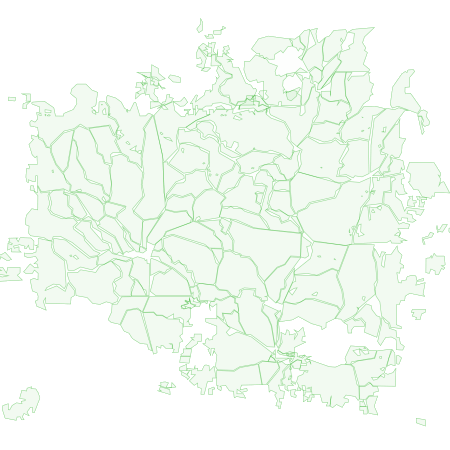
\includegraphics[width=1\textwidth]{images/schema/landuse_example}
      \caption{Landuse (wood) at zoom level 10}
    \end{figure}
\end{minipage}

\begin{figure}[H]
  \centering
  \includegraphics[width=0.8\textwidth]{images/schema/landuse}
  \caption{Landuse layer schema}
\end{figure}

%------------------------------------------------------
\subsection{POI Labels}

\noindent\begin{minipage}[t]{0.48\linewidth}
    \vspace{0pt}
    A point of interest (POI) is a feature bound to a particular point of the map (e.g. churches, schools, tourist attractions, hotels, trees).
    Not all POIs mapped in \osm{} are relevant for a visual map. In order to appear on the map, POIs are required to have at least a name or icon derived by the \textbf{type} field.
    \\\\
    Users shouldn't be overwhelmed with too many point of interest icons. Therefore the field \textbf{localrank} contains an ascending importance rank which can be used by map clients to prioritize important POIs. Very prominent POIs additionally have a scalerank based on their covered \textbf{area}. The rank calculation for POIs works very similar to place label ranking described in \autoref{place_label_rank_calc}.
\end{minipage}
\hfill
\begin{minipage}[t]{0.48\linewidth}
    \vspace{0pt}
    \begin{figure}[H]
        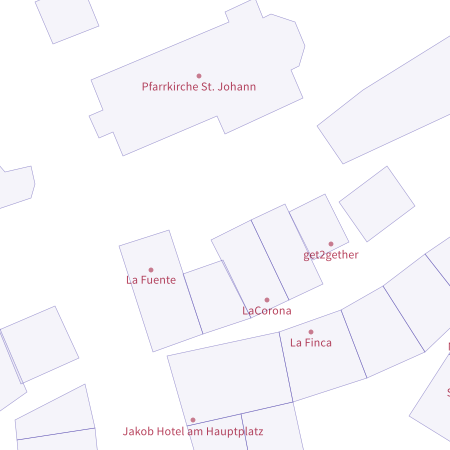
\includegraphics[width=\textwidth]{images/schema/poi_label_example}
        \caption{POI layer on top of building layer}
    \end{figure}
\end{minipage}
\vspace{20pt}
\begin{figure}[h]
  \centering
  \includegraphics[width=0.8\textwidth]{images/schema/poi_label}
  \caption{POI label layer schema}
\end{figure}

%---------------------------------
\subsection{Countries and States}

\noindent\begin{minipage}[t]{0.48\linewidth}
    \vspace{0pt}
    The placement and importance of labels of countries, states and seas matters\cite{12_axismaps.github.io_2015} and is important to get right. 
    Because it is difficult to ensure the quality of these features when importing directly from \osm{}, the labels of countries and states are curated by hand.
    Data from the Overpass API \cite{13_wiki.openstreetmap.org_2015} is converted into GeoJSON and manually edited and enhanced with a label rank to get the best possible label placement and importance ranking.
    This effort is worth it because country and state data changes
    at infrequent intervals.
    Country labels are not present on all zoom levels and are filtered based
    on their \textbf{scalerank} value to show countries like Italy prior to a less important city state like the Vatican.
\end{minipage}
\hfill
\begin{minipage}[t]{0.48\linewidth}
    \vspace{0pt}
    \begin{figure}[H]
        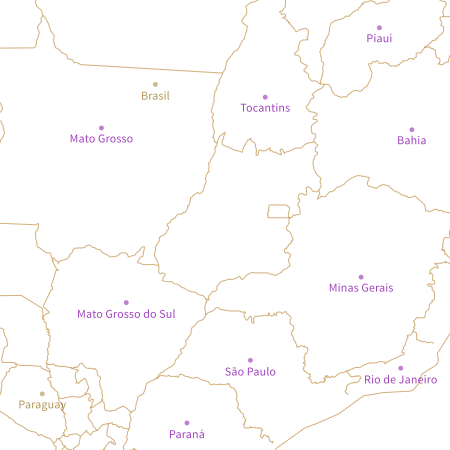
\includegraphics[width=\textwidth]{images/schema/country_state_label_example}
        \caption{Country and state labels around Brasil}
    \end{figure}
\end{minipage}

\begin{figure}[H]
  \centering
  \includegraphics[width=0.8\textwidth]{images/schema/country_state}
  \caption{Country and state layer schema}
\end{figure}

%------------------------------------------------------
\subsection{Places}

\noindent\begin{minipage}[t]{0.48\linewidth}
    \vspace{0pt}
    Place labels are vital for building nice maps with good text hierarchy.
    It is important to show only world cities at low zoom levels and then gradually show more and more local places. Filtering happens via the \textbf{scalerank} and \textbf{localrank} fields in the vector tiles. The \textbf{scalerank} field originates from the \textbf{ne\_10m\_populated\_places} table from NaturalEarth and is merged into the \textbf{place\_point} table. Most place labels are mapped as point in \osm{} except for residential districts and islands for which the centroid of the geometry is used as label point.
    Since place labels are very delicate and important
    every zoom level has custom filters to control which places are relevant.
    The rank calculation for places is explained in \autoref{place_label_rank_calc}.
\end{minipage}
\hfill
\begin{minipage}[t]{0.48\linewidth}
    \begin{figure}[H]
      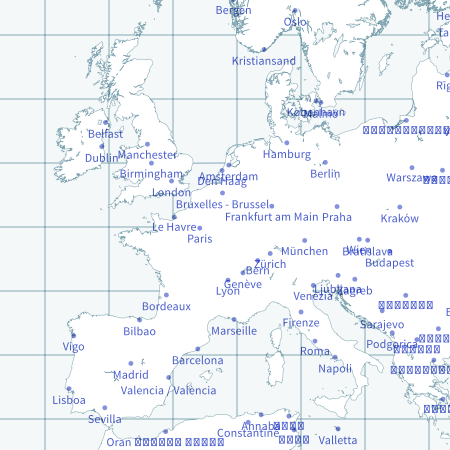
\includegraphics[width=1\textwidth]{images/schema/place_example}
      \caption{Important place labels in Europe}
    \end{figure}
\end{minipage}

\begin{figure}[H]
  \centering
  \includegraphics[width=0.8\textwidth]{images/schema/place_label}
  \caption{Place label layer}
\end{figure}

%------------------------------------------------------
\subsection{Aeroways and Airports}

\noindent\begin{minipage}[t]{0.48\linewidth}
    \vspace{0pt}
    The layer \textbf{aeroway} contains infrastructure regarding air travel. The most common features are airports and their aprons, runways and taxiways. Airports are big landmarks and therefore all features are already present after zoom level 10. The layer consists of polygons and linestrings because runways are often polygons, while taxiways are mostly linestrings.
    The layer \textbf{airport\_label} contains labels of airports (either a point or the centroid of the airport polygon) since airports are important orientation points. The \textbf{scalerank} field describes the importance of the airport based on the covered area and type.
    Airports usually have official abbreviations (either the IATA, FAA, ICAO or custom reference code) that are stored in the \textbf{ref} field.
\end{minipage}
\hfill
\begin{minipage}[t]{0.48\linewidth}
    \vspace{-20pt}
    \begin{figure}[H]
      \centering
      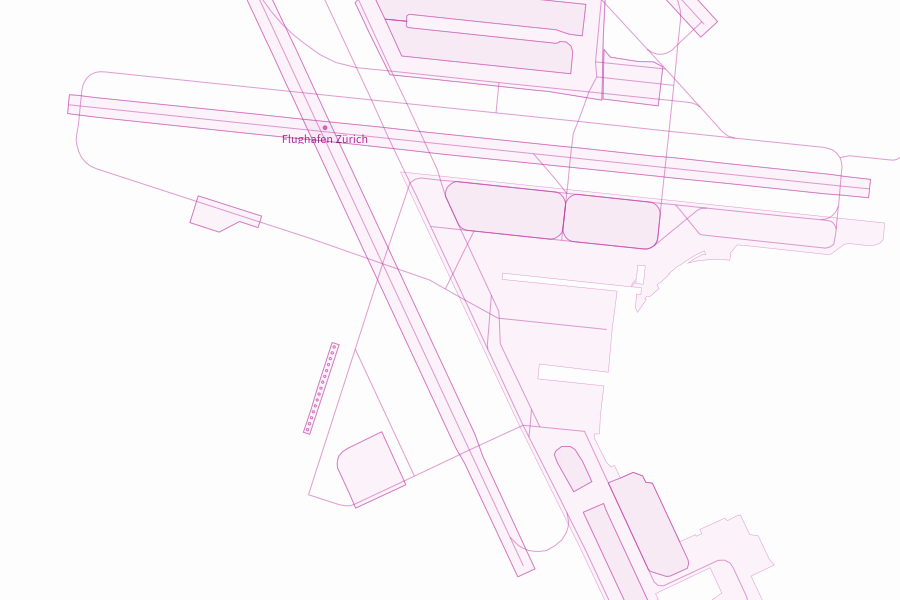
\includegraphics[width=1\textwidth]{images/schema/aeroway_example}
      \caption{Aeroway and airport label layer of Zurich airport}
    \end{figure}
\end{minipage}

\begin{figure}[H]
  \centering
  \includegraphics[width=0.8\textwidth]{images/schema/aeroway}
  \caption{Aeroway layer}
\end{figure}

\begin{figure}[H]
  \centering
  \includegraphics[width=0.8\textwidth]{images/schema/airport}
  \caption{Airport label layer}
\end{figure}

%------------------------------------------------------
\subsection{Oceans, large Lakes and Bays}

\noindent\begin{minipage}[t]{0.48\linewidth}
    \vspace{0pt}
    For oceans, large lakes and bays having a curved label along the body is advantageous because the label does not interfere with other labels like places.
    \\
    Since these features are not available as polygons the label linestrings cannot be calculated but had to be drawn by hand. For the 100+ most important lakes and bays custom linestrings have been drawn. The metadata still originates from \osm{} but the geometries are custom. Since these natural features do not change this does not pose a problem. 
    \\
    The linestrings are filtered ascending for the upper zoom levels based on the \textbf{rank} field and are only shown at low zoom levels 0 to 6.
\end{minipage}
\hfill
\begin{minipage}[t]{0.48\linewidth}
    \vspace{-15pt}
    \begin{figure}[H]
      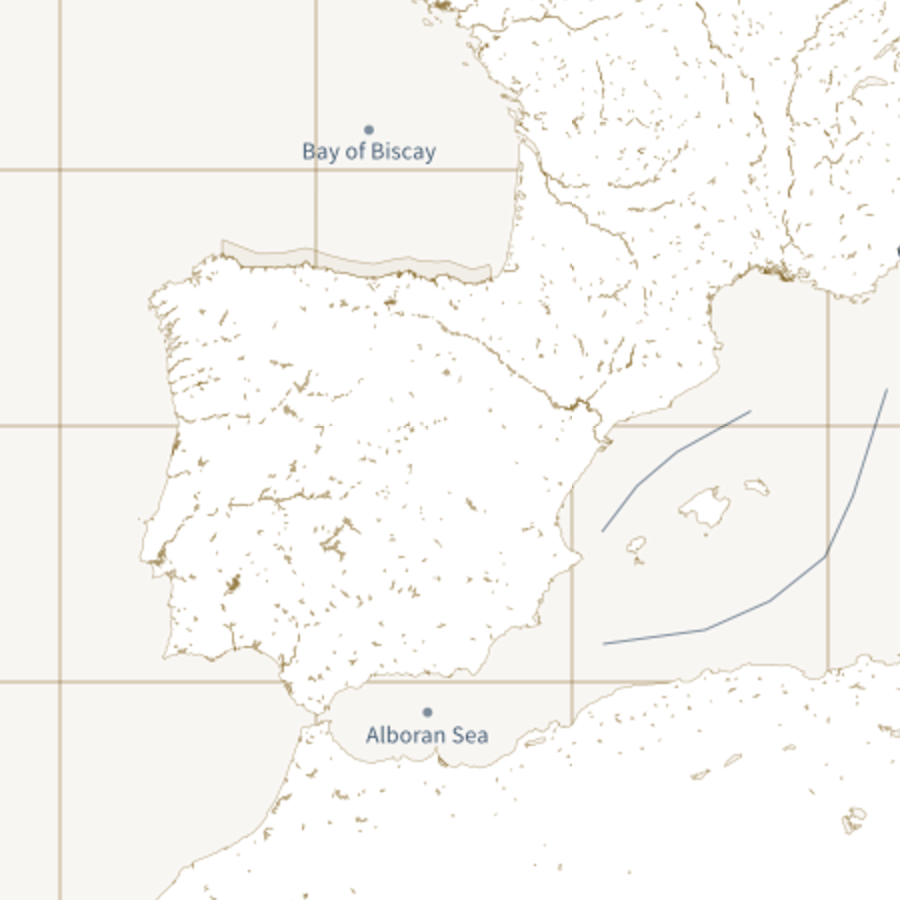
\includegraphics[width=1\textwidth]{images/schema/marine_label_example}
      \caption{Marine label of Mediterranean Sea}
    \end{figure}
\end{minipage}

\begin{figure}[H]
  \centering
  \includegraphics[width=0.8\textwidth]{images/schema/marine_label}
  \caption{Marine label layer}
\end{figure}

%------------------------------------------------------
\subsection{Mountain Peaks}

Mountain peaks are points tagged as mountains and volcanoes with a name and elevation. Because clients only have limited logic capabilities the elevation is calculated in both meters and feet.

\begin{figure}[H]
  \centering
  \includegraphics[width=0.8\textwidth]{images/schema/mountain_peak}
  \caption{Mountain peak label layer}
\end{figure}

%------------------------------------------------------
\subsection{Rail Stations}

Rail stations include railways, metros and tram stations. Since these
public transport features are usually styled differently than other point of
interests they are contained in a separate \textbf{rail\_station\_label\_layer}.

\begin{figure}[H]
  \centering
  \includegraphics[width=0.8\textwidth]{images/schema/rail_station}
  \caption{Rail station label layer}
\end{figure}